
\documentclass[10 pt]{article}



\usepackage{amsthm,amsmath,amssymb,epsf, epsfig, color,enumerate,amssymb,hyperref,ytableau}

\usepackage{tikz}





\newcommand{\G}{{\cal G}}
\newcommand{\EX}{{\cal X}}
\newcommand{\J}{{\cal J}}
\newcommand{\N}{{\mathbb{N}}}
\newcommand{\R}{\mathbb{R}}
\newcommand{\Ho}{{\cal H}}
\newcommand{\M}{{\cal M}}
\newcommand{\Lc}{{\cal L}_3}





\newtheorem{defin}{Definition}[section]
\newtheorem{thm}{Theorem}[section]
\newtheorem{prop}[thm]{Proposition}
\newtheorem{claim}[thm]{Claim}
\newtheorem{remark}[thm]{Remark}
\newtheorem{lemma}[thm]{Lemma}
\newtheorem{con}[thm]{Corollary}
\newtheorem{conj}[thm]{Conjecture}
\newtheorem{exm}[thm]{Example}
\newtheorem{prob}[thm]{Problem}
\newcommand{\arx}[1]{\href{http://arxiv.org/abs/#1}{\texttt{arXiv:#1}}}



\date{}

\title{Mixing Time for Some Adjacent Transposition Markov Chains}

\author{Shahrzad Haddadan, Peter Winkler}

\begin{document}

\maketitle

\begin{abstract}

We prove rapid mixing for certain Markov chains on the set  of permutations on  in which adjacent transpositions
are made with probabilities that depend on the items being transposed.  Typically, when in state , a position  is chosen
uniformly at random, and  and  are swapped with probability depending on  and .
The stationary distributions of such chains appear in various fields of theoretical computer science \cite{Wilson, Self1, Mallow},
and rapid mixing established in the uniform case \cite{Wilson}.

Recently, there has been progress in cases with biased stationary distributions \cite{Benjamini, Dana}, but there are wide classes of
such chains whose mixing time is unknown.  One case of particular interest is what we call the ``gladiator chain,'' in which each number 
is assigned a ``strength''  and when  and  are adjacent and chosen for possible swapping,  comes out on top with probability
.   We obtain a polynomial-time upper bound on mixing time when the gladiators fall into only three strength classes.

A preliminary version of this paper appeared as ``Mixing of Permutations by Biased Transposition'' in STACS 2017 \cite{Stacs}.
 \end{abstract}

\section{Introduction}\label{intro}
For , let  be the set of all permutations of the numbers .  One can think of a permutation as the order
in which a search engine arranges its results \cite{Mallow}, the order in which a self organizing list arranges its items \cite{Self1,Self2},
or the order the playing cards appear after shuffling \cite{Wilson, Diaconis}; each of these suggests different probability distributions on .
Taking samples from such distributions is a useful task which can be tackled using a Markov chain, in particular when dynamic programming approaches
fail to have a polynomial runtime.\footnote{We note here that for the particular case of our study, i.e., gladiators with constant number of
strengths, the dynamic programming approach is efficient. However, the mixing problem is still interesting for at least two reasons:
(1) As discussed in the introduction, a self-organizing list is basically a Markov chain with high mixing time. Thus, analyzing the gladiator
chain is closely related to studying this data structure's performance.  (2) Dynamic programming algorithms would require exponential
time when we have polynomial number of teams. Thus, employing Markov chains could provide an efficient sampling tool in such cases.} 

\smallskip
A natural Markov chain on  picks a number  uniformly at random and from state , puts 
ahead of  with probability . We call such chains \emph{adjacent transposition} Markov chains. 

\medskip 

In this paper, we consider the total variation mixing time, which is defined as the number of steps required before the total variation distance
between the distribution of the current state and stationarity is less than  (where  is some fixed convergence factor).
For Markov chain  we denote this time by , or if , simply by .
 
\smallskip

Jim Fill \cite{FillConj} conjectured that if an adjacent transposition Markov chain is monotone, then it is rapidly mixing.
Monotonicity in this context means that for all  satisfying , , , and 
  \cite{FillConj}. Furthermore, his conjecture asserts ``the simple chain'' whose stationary distribution is uniform
has the highest spectral gap among all monotone adjacent transposition chains.\footnote{ The spectral gap is another measure of mixing.
Here, we are interested in total variation mixing time which, in this case, is within a polynomial factor of the spectral gap.}

\smallskip

Here we provide a brief history of the results  on the adjacent transposition Markov chains.   All of these chains are monotone and rapidly mixing.
Wilson and Benjamini's papers \cite{Wilson, Benjamini} led to Fill's conjecture \cite{FillConj}; Bhakta et al.\ \cite{Dana} verified the conjecture
in two cases.  The current paper, as well as a recent result by Miracle et al. \cite{SaraAmanda}, study the so-called ``gladiator chain'' under
certain conditions, and verify Fill's conjecture in limited cases. We will define the gladiator chain and present a few of its applications
later in this introduction. 

\medskip

 \textbf{1. The simple chain. } In the case where  for all  and , the chain will have a simple description:
Given a permutation , pick two adjacent elements uniformly at random, and flip a fair coin to decide whether to swap them.
We call this chain, whose stationary distribution is uniform, the \emph{simple} chain. Getting precise mixing results for this chain turned
out not to be simple; many papers targeted this problem \cite{Simple1,ComparisonMethodDiaconis}, and finally Wilson \cite{Wilson} showed
the mixing time for this chain is  (that is, he obtained lower and upper bounds within a constant factor).
 
 \smallskip
\textbf{2. The constant-bias chain.} After Wilson's paper, Benjamini et al. \cite{Benjamini} studied the case where  for all ,
and .  The stationary distribution of this chain is the one assigning a probability  proportional to ,
to each  where  is the number of inversions in . This distribution appears in statistics and machine
learning since it is the distribution generated by the ``Mallows model'' \cite{Mallow, Mallow2}.

Benjamini et al. \cite{Benjamini}, showed that the constant biased Markov chain is closely related to another Markov chain known as
the \emph{asymmetric simple exclusion process}, and both chains mix in  steps. We will talk more about exclusion processes
later on in this introduction.

 \smallskip

\textbf{3. ``Choose your weapon" and ``league hierarchy" chains.} The following two special cases were studied by Bhakta et al. \cite{Dana}.
In the \emph {choose your weapon chain}  is only dependent on , and the \emph{league hierarchy chain} is given by a binary tree
 with  leaves. Each interior node  of  is labeled with some probability , and the leaves are labeled by numbers
. The probability of putting  ahead of  for  is equal to  where  is the node that
is the lowest common ancestor of  and  in . Bhakta et al.\ showed that the choose your weapon chain mixes in 
steps and the league hierarchy chain in  steps. 
\medskip

Here we are interested in \emph{gladiator} chains, which constitute a subclass of the monotone adjacent transposition chains. Gladiator chains
have connections to self organizing lists, and were introduced by Jim Fill.
\medskip

Fill was interested in probabilistic analysis of algorithms for \emph{self-organizing lists} (SOLs). Self-organizing lists are data structures 
that facilitate linear searching in a list of records; the objective of a self-organizing list is to sort the records in non-decreasing order
of their access frequencies \cite{Self1}. Since these frequencies are not known in advance, an SOL algorithm aims to move a particular
record ahead in the list when access on that record is requested. There are two widely used SOL algorithms: the \emph{move ahead one}
algorithm (MA1) and the \emph{move to  front }algorithm (MTF). In MA1, if the current state of the list is
 and the th record is requested for access,  it will go ahead in the list only one
position and the list will be modified to .  In MTF it will go to the front and the
list will be modified to . It appears that  MA1 should perform better than MTF when the
list is almost sorted and worse when the low frequency records are standing in front; although this has been confirmed by simulations,
it has not been analytically confirmed \cite{Self2}.  Considering the adjacent transposition Markov chain corresponding to MA1, Fill shows
\cite{FillConj} that there are cases in which the chain is not rapidly mixing. Hence, he poses the question of sampling from the stationary
distribution of MA1, and he introduces the gladiator chain which has the same stationary distribution as MA1 and seems to be rapidly mixing for arbitrary
choice of parameters.

In the gladiator chain, each element  can be thought of as a gladiator with strength . Every permutation of numbers 
can be thought of as a ranking of gladiators. In each step of Markov chains we choose  uniformly at random, i.e., we choose
adjacent gladiators  and . These gladiators will fight over their position in ranking. With probability
, gladiator  will be the winner of the game and will be placed ahead of  in  if he isn't already.
With probability ,  is put ahead of .  If Fill's conjecture holds, gladiator chains must mix rapidly. 
 \medskip
 
 
 
\textbf{Exclusion processes.} A related Markov chain which has received a lot of attention is the \emph{exclusion process} (\cite{exc1, exc2}).
In this chain we have a graph    and   particles  on the vertices of . The sample space is the
set containing all the different placements of the  particles on vertices of . At each step of the Markov chain we pick a vertex 
uniformly at random with probability   and  one of its adjacent vertices  with probability  . If there is a
particle in one of the vertices and not the other one, we swap the position of the particle with a constant probability . We are interested
in the \emph{linear} exclusion process when the graph is a finite path with  vertices.  As mentioned before, the linear exclusion process
was studied by Benjamini et al.\ \cite{Benjamini} and is known to be mixing in time .\footnote{Benjamini et al.\ use this
result to prove that the constant biased adjacent transposition chain is rapidly mixing.} Later, Greenberg et al.\ \cite{Greenberg}
presented a simpler proof. 

 \medskip
\textbf{Our Contribution.}
We study the gladiator chain when the gladiators fall into a constant number of teams, gladiators in each team having the same strength
(Definition \ref{defteams}).  We then extend the definition of linear exclusion process (studied by Benjamini et al.) by allowing particles
of different types to swap their positions on a line. We call this new chain a \emph{linear particle system} (Definition \ref{defparts}).
We will show that mixing results for linear particle systems can produce mixing results for gladiator chains (Theorem \ref{reduction}). 

In particular, we study the linear particle system in which there are three particle types, and in Theorem \ref{mainthm} we extend
Benjamini et al.'s result by  showing the three particle system mixes rapidly. Having Theorem \ref{mainthm} we conclude that the
following adjacent transposition chains mix rapidly, and hence confirming Fill's conjecture in these cases: The gladiator chain
when gladiators fall into three teams of same-strength gladiators; and the league hierarchy chain for ternary trees
(extending Bhakta et al.'s work \cite{Dana}). 
\medskip

\textbf{Remark.} We believe linear particle systems, like exclusion processes, are interesting Markov chains that may appear as components
of other Markov chains, and thus would facilitate studying mixing times of other chains. For instance, in Section \ref{trees} of this paper,
by using Theorem \ref{mainthm} we extend a result about binary trees to ternary trees.  As another example, we remind the reader of the
correspondence between the exclusion process and the Markov chains on the lattice paths in an  rectangular lattice
(Figure \ref{figlatticepath}). Similarly, there is a correspondence between the linear particle systems having  particles and the lattice
paths in dimensional lattices (Figure \ref{figlatticepath}). Some Markov chains defined on lattice paths in a dimensional rectangle
have already been studied by Greenberg et al.\ \cite{Greenberg}.

\smallskip

We remark here that following our result in STACS 2017 \cite{Stacs}, Miracle et al.\ \cite{SaraAmanda} studied the mixing time of
linear particle system when the number of particles is a constant , and showed the mixing time is upper bounded by .
With different techniques from ours, they  prove the mixing time of gladiator chains with a constant number of teams is upper bounded
by . The mixing time for linear particle systems and gladiator chains with teams, remains an open problem in the cases
in which the number of particle types or teams is more than a constant. 

\begin{figure}[!h]\label{figlatticepath}
\smallskip
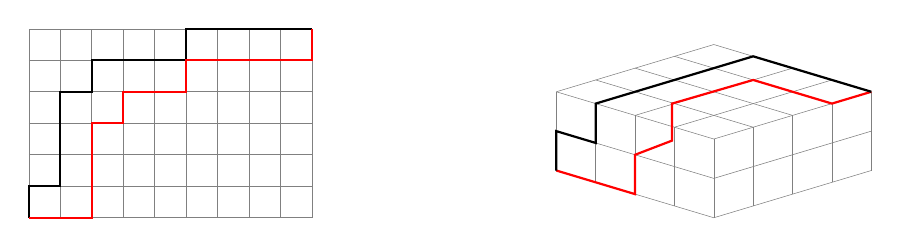
\begin{tikzpicture}
\draw[step=0.4cm,gray,very thin] (-1.2,-1.2) grid (2.4,1.2);
\draw[thick](-1.2,-1.2) --(-1.2,-0.8)--(-0.8,-0.8)--(-0.8,-0.4)--(-0.8,0.0)--(-0.8,0.4)--(-0.4,0.4)
--(-0.4,0.8) --(0.0,0.8)--(0.4,0.8)--(0.8,0.8)--(0.8,1.2)--(1.2,1.2)--(1.6,1.2)--(1.8,1.2)--(2.4,1.2) ;
\draw[red,thick](-1.2,-1.2) --(-0.8,-1.2)--(-0.4,-1.2)--(-0.4,-0.8)--(-0.4,-0.4)--(-0.4,0.0)--(0.0,0.0)
--(-0.0,0.4) --(0.4,0.4)--(0.8,0.4)--(0.8,0.8)--(1.2,0.8)--(1.6,0.8)--(2.0,0.8)--(2.4,0.8)--(2.4,1.2);
\draw[step=0.4cm, gray, very thin] (5.5,-0.6) -- (7.5,-1.2)--(9.5,-0.6);
\draw[step=0.4cm, gray, very thin] (5.5,-0.1) -- (7.5,-0.7)--(9.5,-0.1);
\draw[step=0.4cm, gray, very thin] (5.5,0.4) -- (7.5,-0.2)--(9.5,0.4);
\draw[step=0.4cm, gray, very thin] (5.5,0.4) -- (7.5,1.0)--(9.5,0.4);
\draw[step=0.4cm, gray, very thin]  (6.0,0.55)-- (8.0,-0.05);
\draw[step=0.4cm, gray, very thin]  (6.5,0.70)-- (8.5,0.10);
\draw[step=0.4cm, gray, very thin]  (7.0,0.85)-- (9.0,0.25);
\draw[step=0.4cm, gray, very thin]  (6.0,0.25)--(8.0,0.85);
\draw[step=0.4cm, gray, very thin]  (6.5,0.1)--(8.5,0.7);
\draw[step=0.4cm, gray, very thin]  (7.0,-0.05)--(9,0.55);

\draw[step=0.4cm, gray, very thin]  (7.5,-0.2)--(7.5,-1.2);
\draw[step=0.4cm, gray, very thin]  (7.0,-0.05)--(7.0,-1.05);
\draw[step=0.4cm, gray, very thin]  (8.0,-0.05)--(8.0,-1.05);
\draw[step=0.4cm, gray, very thin]  (6.5,0.10)--(6.5,-0.90);
\draw[step=0.4cm, gray, very thin]  (8.5,0.10)--(8.5,-0.90);
\draw[step=0.4cm, gray, very thin]  (6.0,0.25)--(6.0,-0.75);
\draw[step=0.4cm, gray, very thin]  (9.0,0.25)--(9.0,-0.75);
\draw[step=0.4cm, gray, very thin]  (5.5,0.40)--(5.5,-0.60);
\draw[step=0.4cm, gray, very thin]  (9.5,0.40)--(9.5,-0.60);
\draw[red,thick](5.5,-0.6)--(6.0,-0.75)--(6.5,-0.90)--(6.5,-0.4)--(6.97,-0.22)--(6.97,0.25)--
(8,0.55)--(9.0,0.25)--(9.5,0.40);
\draw[black,thick](5.5,-0.6)--(5.5,-0.1)--(6.0,-0.25)--(6.0,0.25)--(8.0,0.85)--(9.5,0.40);
\end{tikzpicture}
\caption{The correspondence between lattice paths and linear particle systems:
The  picture on the left  illustrates two paths in a two dimensional lattice; the red one corresponds to
001110100100001 and the black one corresponds to 10110100010000.
The picture on the right illustrates two paths in a three dimensional lattice; the red one corresponds to
0012122002 and the black one corresponds to 1012222000.
}
\end{figure}


\medskip
Definitions and results are presented in Section \ref{Section1}, along with the correspondence between the gladiator chains and the
linear particle systems. Section \ref{proof} contains the proof that the linear three-type system mixes rapidly under certain conditions.
In Section \ref{trees}, we discuss the league hierarchy chain and our result for ternary trees.  

\section{Definitions and Results}\label{Section1}



\begin{defin}\textbf{Gladiator chain} (Playing in teams).\label{defteams}
Consider the Markov chain  on state space  that has the following properties: The set   (i.e. gladiators)  can be  partitioned
into subsets:  ( teams). We have the following strength function: ,  iff .
At each step of Markov chain,  we choose  uniformly at random. Given that we are at state , and , we put  ahead of  with probability .  We denote a gladiator chain having  gladiators
playing in  teams by .\footnote{Although the notation  would be more precise ( being cardinality
of ), we avoid using it for simplicity and also because our analysis is not dependent on .}

\end{defin}


This is a reversible Markov chain and the stationary distribution  is
\label{stationary}


Note that by writing  we mean gladiator  is located at position  in . By writing 
 we are referring to the position of gladiator  in the permutation . We use this notation throughout the text
and for permutations presenting both gladiators and particles. 


\begin{defin}\textbf{Linear particle systems.}\label{defparts}
Assume we have  types of particles and of each type , we have  indistinguishable copies. Let . 
Let  be the state space containing all the different linear arrangements of these  particles. 
If the current state of the Markov chain is , choose  uniformly at random.  Let  be of type 
and  be of type . If  do nothing. Otherwise, put  ahead of  w.p.\  and
put  ahead of  w.p.\ .  We denote the linear particle system having  particles of
 different types by .
\end{defin}
This chain  is also a reversible Markov chain. In the special case where   the stationary distribution  is
\label{eq2}

\begin{prop}
By regarding gladiators of equal strength as indistinguishable particles, we associate to any gladiator system a linear particle system.
\end{prop}

Note that the state space of the gladiator system has cardinality  for  different gladiators but the linear particle system has only
 states, since particles of the same type are indistinguishable. Thus, . The following theorem,
whose proof will be presented later, shows the connection between the mixing times of the two chains.
\begin{thm}\label{reduction}
Let  and  be respectively the mixing times for a linear particle system and its corresponding gladiator chain.
Then, .
\end{thm}


Our main result, which extends the results of Benjamini et al.\ \cite{Benjamini} on exclusion processes, is the following:

\begin{thm}\label{mainthm}
Let  be a linear particle system of Definition \ref{defparts}, having particles of type A, B and C.
Assume that we have strength functions assigned to each particle type, namely , and thus swapping probabilities
,  and .
If , then the mixing time of  satisfies 

\end{thm}

\begin{remark}
The condition  comes from the following simple bound on -binomials that we later prove in Lemma~\ref{qlemma}: 
If   then, 

Better bounds on -binomials would allow the result to be improved.
\end{remark}

We will prove Theorem \ref{mainthm} in Section \ref{proof}.
Having Theorem \ref{mainthm}, we deduce the following case of Fill's conjecture: 
 
 \begin{con}
The mixing time of  satisfies , provided  and
, where  is the strongest playing team among the three, and  the gladiators in team  are stronger than the gladiators in team .
\end{con} 
 
\begin{proof}
From Theorems \ref{mainthm} and \ref{reduction}. 
\end{proof}
 
We present the following corollary of Theorem \ref{mainthm} here and discuss it in full detail later in Section \ref{trees}.
 
\begin{con}(League hierarchies for ternary trees)\label{LeagueHi}
Let  be a ternary tree  with  leaves. The children of each interior node  are labeled with labels , , and ,
and each internal node has three strength values , , and . The leaves are labeled by numbers .
The probability of putting  ahead of  for  is equal to  where  is the node
that is the lowest common ancestor of  and  in , and  is the child of  which is an ancestor of ,
and  is the child of  which is an ancestor of . If for each , , , and 
satisfy the conditions in Theorem \ref{mainthm}, then the mixing time of the league hierarchy chain is bounded by .
\end{con} 

 
 \medskip
  
We finish this section by proving Theorem \ref{reduction}.
 
\subsection{Gladiators and Particles (Proof of Theorem \ref{reduction})}

Consider the gladiator chain  for arbitrary  being the number of gladiators  and  the number of teams.
Assume that we have  gladiators on team ; hence, .  At each step of the chain, one of two things is happening: 
\begin{enumerate}
\item Whisking: gladiators of the same team are fighting. 
\item Sifting:  gladiators of different teams are fighting.
\end{enumerate}
If we were restricted to  whisking steps the chain would be equivalent to a product of several simple chains analyzed by Wilson \cite{Wilson}.
If we were restricted to sifting steps the chain would be the linear particle system chain introduced in Definition \ref{defparts}. 
In order to study the mixing time of the gladiator chain we  analyze sifting and whisking steps separately, and then we employ the
following decomposition theorem: 

\begin{thm}\label{decom}  \textbf{Decomposition Theorem \cite{Decomposition}.}
Let  be a Markov chain on state space  partitioned into .
For each , let  be the restriction of  to  that rejects  moves  going outside of .
Let  for . We define the Markov chain  on
state space  as follows: ,
where  and  are transition probabilities of  and  respectively. 
Then 

\end{thm}
 To apply the decomposition theorem, we partition  to  for all choices of , each  being the set of all permutations in
 in which all the gladiators corresponding to particle  preserve the ordering associated to them by .
The restriction of  to  is equivalent to .
We define  to be the Markov chain on  with the following transition probabilities: 


where   and  are only different in swapping   and st elements and
 iff  and st copies of particle  are adjacent in  and swapped in . 
Moreover, we observe that:
 
We can verify the above equation by the following reasoning: consider an arbitrary permutation
 in which th and st copies of particle  are not adjacent.
We can map  to two other permutations  and  where in  we take the the th copy of particle  down to make it
adjacent to the st copy, and in   we take the the st copy of particle  up to make it adjacent to the th copy.
We will have , and hence one of  or  will be larger than .
This mapping is in worst case  to , hence the above equation holds.  

Having the above observations, we realize  is the product of  adjacent transposition Markov chains, and in each of these
Markov chains we swap two adjacent elements with probability at least . Let these chains be .
By comparing the conductance (for more information about conductance, see \cite{MCBook}) of this chain to the simple chain analyzed
by Wilson \cite{Wilson}, for each  we will have . 
We use the following Theorem of \cite{Dana}:

\begin{thm}\label{product}
If   is a product of  independent Markov chains 
and it updates each   with probability , then

\end{thm}

Plugging in , we have . Summing up and employing the Decomposition Theorem,



\section{ Three-Particle Systems (Proof of the Main Theorem)}\label{proof}

In this section we prove Theorem \ref{mainthm} which states that  if 
.

Assume that we have  copies of particle ,  copies of particle , and  copies of particle .
We denote the set containing all the different arrangements of these particles by .
We introduce another Markov chain  on the same sample space .
Using the comparison method (see \cite{compare}) we will show that the mixing times of  and  are related.

Then we will use the path congestion technique to show  mixes in polynomial time, and hence we deduce Theorem \ref{mainthm}.



\textbf{Notation.} We denote the substring  by , and by  we refer
to a string which is  copies of particle . 

\begin{defin}
Let   be a Markov chain on state space  and . If the current state is ,
we choose natural numbers  uniformly at random and swap them following these rules (Figure \ref{figJH}):
\end{defin}

\begin{enumerate}
\item If   and in  or vice versa and .  Then,
put  and   in increasing order of their strength w.p.\ .
With probability , put them in decreasing order. We call this move a \emph{Jump} and we denote
it by  if  and ; and  for vice versa. 

\item If  and     or  if  and  .
Then, put  and  in increasing order of their strength w.p. .
With probability , put them in decreasing order. We call this move a \emph{Hop},
and we denote it by   if   and ; and  for vice versa.
Similar rules and notation apply when swapping  and . 
\item Else, do nothing.
\end{enumerate}

\begin{figure}[!h]

\centerline{\resizebox{0.7 \linewidth}{!}{\includegraphics{figure2}}}
\caption{Jumps and Hops are the transitions  in the Markov chain .}\label{figJH}
\end{figure}



It can be easily checked that  is reversible and its stationary distribution is the  in Equation \ref{eq2}.

\begin{lemma}\label{lem1}

\end{lemma}

\begin{proof}

We use the comparison technique\footnote{
The comparison method was introduced by Diaconis and Saloff-Coste \cite{ComparisonMethodDiaconis}; Randall and Tetali extended it and employed
it for analysis of Glauber dynamics \cite{compare}.  For more information about this method we encourage the reader to refer to \cite{MCBook}.
}
 in the proof of Lemma \ref{lem1} (see \cite{ComparisonMethodDiaconis, compare}). To any edge  in , we assign a path
from  to  in .  Let  be a move in  which swaps particles  and  located at positions
 and  in an arrangement. To   making  in , we correspond the following path in :
. We denote this path by ,
and the set contaning all such paths by  . 
Similarly, to   making  in , we correspond the following path in :
. We denote this path by , and the set contaning all such
paths by . Let .


We now bound the congestion placed by  on edges of .
Consider an arbitrary   making swap  and assume  where  and
 are particles different from . For any  and  in  if  then,
there must be   and  such that  corresponds to  or
to . Thus, the congestion placed on  only by paths in  is:





We can similarly show that the congestion placed on  by  is less than , where  is the length of the
arrangements or total number of particles. For each , let  be the congestion  places on .
We will have .  We also know , where  (we consider 
to be a constant). Hence, employing the Comparison Theorem we have


\end{proof}

Having the above connection it suffices to bound the mixing time of . In the rest of this section our goal is to bound
. We use the path congestion theorem, which is stated below.  In particular,
for any two arbitrary states ,  we introduce a path .
Then we show that none of the edges of the Markov chain  is congested heavily by these paths.
Formally, we employ Theorem \ref{canonicalPaths} and in Theorem \ref{big} we show that .

\newpage
\begin{thm}(Canonical Paths Theorem \cite{Permanent})\label{canonicalPaths}

Let  be a Markov chain with stationary distribution  and   the set of the edges in its underlying graph. 
For any two states  and  in the state space  we define a path .
The congestion factor for any edge  is denoted by  and is defined by
 . We can bound the mixing time of  using the congestion factor:

where ,  and  is the convergence parameter. 
\end{thm}

\textbf{The Paths.}
For each , we introduce the following path in  from  to : We partition 
and  to  blocks; the end points of these blocks are locations of s in . For instance if in , the first 
is located at position  and the second  is located at position  then, the first block in both  and  is ,
and the second is . Starting from the first block, we change each block in two steps, first we use Jump moves and change
the relative position of  and s in  to become in the order in which they appear in . Then, we bring the 
in that block to its location in . Formally, we repeat the following loop:
\medskip

\textbf{Notation.} By saying , we mean the th copy of particle  is located at position  in . 

\noindent 
Starting from , we repeat the following steps until  is reached.

Initially, let . 
\begin{enumerate}
\item Let . We define the  th \emph{block} of  and  to be the substring starting from  and ending in .
Note that in , each blocks starts right after a  and ends with a . In the th iteration, the goal is to change
 until , i.e. the first  blocks equal in  and .

\item Using Jumps, and starting from the lowest index , we bring particles  or  down until  and  particles in the block
 have the same order in  and .
\item We use Hops and bring the th  in  to . In this process, we may need to bring several copies of particle
 out of the th block in . In that case, we choose a random ordering of s and move them with respect to that order
(details explained in the proof of Claim \ref{PathClaim}).
\item Set .
\item Increment .
\end{enumerate}


\begin{figure}[h]
\noindent
\begin{tiny}


\begin{tabular}{ccccccccr}
\mbox{1st iteration:} &\quad&\quad&\quad\quad\quad\quad\quad\quad\quad\quad\quad\quad\quad\quad\quad\quad\quad\quad\quad&\mbox{2nd iteration:}&\quad&3rd iteration:\\
\end{tabular}

\hspace*{-0.3cm}
\begin{tabular}{rcccccccccccccc}
C&&C&& C&&C&&C&&C&&\textcolor{red}{C}&&A\\
A& &A&& A&&A&&A&&{A}&&\textcolor{red}{A}&&C\\
B&&B& &B&&B&&B&&\textcolor{red}{B}&&{C}&&C\\
C&&C&&\textcolor{red}{ C}&&C&&C&&\textcolor{red}{C}&&B&&B\\
A&\mbox{\tiny Jump}&A&\mbox{\tiny Jump}&\textcolor{red}{ A}&\mbox{\tiny Jump}&A&\mbox{\tiny Hop}&\textcolor{red}{A}&\mbox{\tiny Hop}&B&\mbox{\tiny Hop}&B&\mbox{\tiny Jump}&B\\
{C}&&\textcolor{red}{C}&& A&&\textcolor{red}{A}&&\textcolor{red}{B}&&A&&A&&A\\
B&\mbox{\tiny Step 1}&B&\mbox{\tiny Step 1}& B&\mbox{\tiny Step 1}&\textcolor{red}{B}&\mbox{\tiny Step 2}&A&\mbox{\tiny Step 2}&A&\mbox{ \tiny Step 2}&A&\mbox{\tiny Step 1}&A\\
\textcolor{red}{C}&& \textcolor{red}{A}&&C&&C&&C&&C&&C&&C\\
\textcolor{red}{A}&& C&&C &&C&&C&&C&&C&&C 

\end{tabular}
\caption{We use the path congestion technique to bound . In each iteration we fix a block in  until  is reached.}
\end{tiny}
\end{figure}







\begin{claim}\label{PathClaim}
 Let  be the set of paths defined as above. Then, for any arbitrary edge  in
the Markov chain  the congestion , defined in Theorem \ref{canonicalPaths} satisfies .

\end{claim}

We present a roadmap to the proof of the above claim before providing details.
\smallskip

In order to verify the claim, we analyze the congestion of  Jump and Hop edges separately. In both of the analyses, we consider an
edge , and to any  such that  we assign a .
The reverse image of  could be a subset of . However, using
binomials\footnote{More information about -binomials can be found in Richard Stanley's course ``Topics in Algebraic Combinatorics,''
Chapter 6 (see \cite{Stanley}). }
we show that  is bounded by a polynomial function of
 multiplied by , and then we conclude the claim. A key factor of our analysis is the use of -binomials.
Note the following observations:
Assume that we have no copies of particle ,  copies of , and  copies of particle . Let  be the
arrangement with maximum stationary probability, i.e. . Note that for each , ,
where  is the number of transpositions needed to get from  to . For a constant , the number of s requiring 
transpositions is equal to the number of integer partitions of  fitting  in an  rectangle (see Figure \ref{qbin}). Thus:
 
\begin{figure}[!h]




\caption{Correspondence of partition functions with q-binomials: There are three integer partitions of 9 that fit into a 34 rectangle,
and there are three arrangements of gladiators in  with . In other wors, the coefficient
of  in  equals 3.}\label{qbin}
\end{figure}
We will use the following lemma in our proof:
\begin{lemma}\label{qlemma}
 If  then, .
\end{lemma}
\begin{proof}


\end{proof}


\begin{proof}[Proof of Claim~\ref{PathClaim}]


Consider an edge  corresponding to . Assume that , 
(remember the notation  meaning the th copy of particle  is located at position  in ),
i.e., this edge is swapping the th  with the th  in .


It follows from the  way we set the paths that, for some , ,
and  for some . 
The preceding blocks of  have been changed in accordance with , and the succeeding blocks of  have
not been changed yet, hence they resemble  blocks.
Therefore we have  and  (see Figure \ref{Move2fig}).

We define the function  as follows: 
For any  satisfying , let 
(the symbol  denotes concatenation). Since the arrangements of particles is changing, we may have
. For instance we may have  and
 but  or  or .
However, we know , which means there is a way to substitute the particles
in  to change  to  so that .
We call this stage the substitution stage, in which we identify the particle or particles with extra copies in ,
and we substitute the lowest copies of them with inadequate particles and produce .
Then, we define .
For instance, if  , then substitute the lowest  copies of  and
 with s, and produce .
The substitution stage will cause a \emph{substitution cost}, we denote the substitution cost by ,
and define it as: , where  . Note that
if we make  substitutions, the substitution cost is at most .
To make the analysis simpler we only analyze the worst case in which we assume we have substituted 
s with s in . This assumption also means that in  we have  more s and  fewer s than in .  

\begin{figure}[!ht]

\centerline{\resizebox{0.7\linewidth}{!}{\includegraphics{figure4}}}

\caption{We define . To produce  we first concatenate  and , then
substitute some particles.}\label{Move2fig}
\end{figure}



Consider  such that . Let . We have, 

where the later term is the substitution cost, and .
Having  we will get:





Let   be the set of all s with  substitutions. We  have:


Let   be the  arrangement that we get from replacing the lowest  copies of particle  with copies of particle 
in  . We have:
, where , and 
M_t(\alpha)

\begin{figure}[!ht]

\centerline{\resizebox{0.4\linewidth}{!}{\includegraphics{figure3}}}

\caption{We obtain  from  and then take the sum over all s (Equation \ref{eq3}). }
\end{figure}\label{fig6}
\smallskip
Note that ,   being .
This inequality holds because  and (See Figure 6).

Moreover, , where  is the number of s in  and .

\smallskip
Putting all of the above inequalities together, we will have that each edge of Jump is only congested by:



So far, we showed that any Jump edge is only congested by a factor of a polynomial function of . 
Consider  an edge corresponding to a Hop, namely . We denote this edge by . Assume we are swapping  and .

\medskip

Consider a state  traversing  to get to , and assume we traversed  while fixing block .
Since we are making a Hop,  s and s in the block are fixed according to , and we are  bringing the th   to its position in .

\medskip

Before we proceed to the proof there is a subtlety about using a Hop that needs to be explained. If  has to go down to reach
its position in   or if there is only one copy of it in the block there is no complication. 
Let's assume we have  copies of particle  in . All of the  copies of  should move up and stand out
of block  to reach their position in . In order to accomplish this, we choose a subset  of
 uniformly at random and we move the elements of  in decreasing order of their index out of the block.  

\smallskip

Assume, when going from  to  we used   and in  we have  copies of particle :
 and swapping    with the next .  We have,
, , and for any , if
. 
The following information about  can be determined by examining  and : 
while  may contain any of . Therefore, among the random paths connecting  to ,
there are  subsets traversing through  and hence the congestion they place on 
 is .

 \smallskip

To bound   for each  we introduce correspondence 
  satisfying:

where  is the number of s in  and 

Let  and  be two ends of a path traversing through  . We define ;
to verify Equation \ref{eq4}, take . We have

Thus,

where   is the following arrangement: .
We have . Hence, 


Since we have  s with undecided position between  other elements we have , where . Thus, we have .  Hence, the congestion placed on  is:



Summing up, we showed that for any edge , .

 \end{proof}
 
Having the above claim, we now use the path congestion Theorem (Theorem \ref{canonicalPaths}) to bound :
 \begin{thm}\label{big}
If , then . 
\end{thm}
\begin{proof}

Since ,  being maximum of  and , we can  apply Theorem \ref{canonicalPaths} and we will have,




\end{proof}


Finally, from Lemma \ref{lem1} and Theorem \ref{big} we conclude Theorem \ref{mainthm}.

\section{League Hierarchies for Trenary Trees.}\label{trees}
 
As mentioned earlier in Section \ref{intro}, the \emph{league hierarchies} are a class of monotone adjacent transposition Markov chains and
were introduced by Bhakta et al.\ (SODA 2014) \cite{Dana} for binary trees. Here we extend their definition to trenary trees. 
   
\begin{defin}\textbf{(League hierarchies for ternary trees).} \label{LeagueHiDef}
Consider a ternary tree whose leaves are labeled by , and inside each interior node  there are three numbers
 satisfying :
.
We define the Markov chain  on  as follows.  In state ,  is chosen uniformly at random and
 and  are swapped with probability . The s are defined in accordance with
the tree structure.  For each  , the probability if swapping  is equal to ; , 
being the lowest common ancestor of the leaves labeled   and , and  being one of  depending respectively on whether
they are in the right, left or central subtree rooted at .
 \end{defin}
 
 
\begin{figure}[!h]\label{figlatticepath}
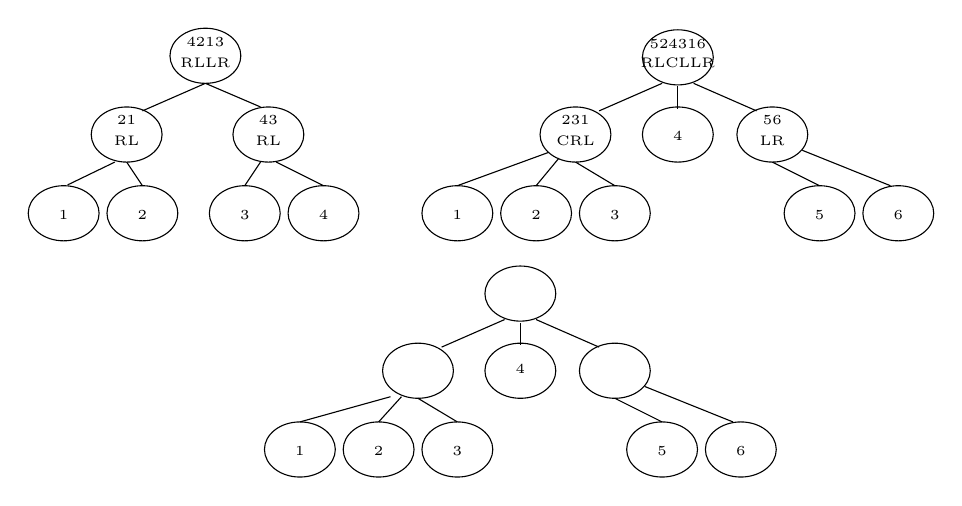
\begin{tikzpicture}\label{fig7}


\draw (4,4) ellipse (4.5mm and 3.5 mm);
\node[above] at (4,4) {\tiny 4213};
\node[below] at (4,4.1) {\tiny RLLR};


\draw (3,3) ellipse (4.5mm and 3.5 mm);
\node[above] at (3,3) {\tiny 21};
\node[below] at (3,3.1) {\tiny RL};


\draw (4.8,3) ellipse (4.5mm and 3.5 mm);
\node[above] at (4.8,3) {\tiny 43};
\node[below] at (4.8,3.1) {\tiny RL};



\draw (4.5,2) ellipse (4.5mm and 3.5 mm);
\node[above] at (4.5,1.8) {\tiny 3};

\draw (5.5,2) ellipse (4.5mm and 3.5 mm);
\node[above] at (5.5,1.8) {\tiny 4};

\draw (2.2,2) ellipse (4.5mm and 3.5 mm);
\node[above] at (2.2,1.8) {\tiny 1};

\draw (3.2,2) ellipse (4.5mm and 3.5 mm);
\node[above] at (3.2,1.8) {\tiny 2};


\draw (4.7,3.35) -- (4,3.65);
\draw (3.2,3.3) -- (4,3.65);


\draw (5.5,2.35) -- (4.9,2.65);
\draw (4.5,2.35) -- (4.7,2.65);
\draw (3.2,2.35) -- (3,2.65);
\draw (2.25,2.36) -- (2.85,2.65);



\draw (7.2,2) ellipse (4.5mm and 3.5 mm);
\node[above] at (7.2,1.8) {\tiny 1};

\draw (8.2,2) ellipse (4.5mm and 3.5 mm);
\node[above] at (8.2,1.8) {\tiny 2};

\draw (9.2,2) ellipse (4.5mm and 3.5 mm);
\node[above] at (9.2,1.8) {\tiny 3};

\draw (10,3.98) ellipse (4.5mm and 3.5 mm);
\node[above] at (10,3.97) {\tiny 524316};
\node[below] at (10,4.1) {\tiny RLCLLR};


\draw (10,3) ellipse (4.5mm and 3.5 mm);
\draw (10,3.33) -- (10,3.61);
\node[above] at (10,2.8) {\tiny 4};

\draw (11.8,2) ellipse (4.5mm and 3.5 mm);
\node[above] at (11.8,1.8) {\tiny 5};

\draw (12.8,2) ellipse (4.5mm and 3.5 mm);
\node[above] at (12.8,1.8) {\tiny 6};


\draw (8.7,3) ellipse (4.5mm and 3.5 mm);
\node[above] at (8.7,3) {\tiny 231};
\node[below] at (8.7,3.1) {\tiny CRL};


\draw (11.2,3) ellipse (4.5mm and 3.5 mm);
\node[above] at (11.2,3) {\tiny 56};
\node[below] at (11.2,3.1) {\tiny LR};



\draw (9,3.3) -- (9.8,3.65);
\draw (11,3.3) -- (10.2,3.65);

\draw (7.2,2.35) -- (8.35,2.77);
\draw (8.2,2.35) -- (8.49,2.7);
\draw (9.2,2.35) -- (8.7,2.65);
\draw (11.8,2.35) -- (11.2,2.65);
\draw (12.7,2.35) -- (11.58,2.8);




\draw (5.2,-1) ellipse (4.5mm and 3.5 mm);
\node[above] at (5.2,-1.2) {\tiny 1};

\draw (6.2,-1) ellipse (4.5mm and 3.5 mm);
\node[above] at (6.2,-1.2) {\tiny 2};

\draw (7.2,-1) ellipse (4.5mm and 3.5 mm);
\node[above] at (7.2,-1.2) {\tiny 3};

\draw (8,0.98) ellipse (4.5mm and 3.5 mm);
\node[below] at (8,0.2) {\tiny 4};



\draw (8,0) ellipse (4.5mm and 3.5 mm);
\draw (8,0.33) -- (8,0.61);


\draw (9.8,-1) ellipse (4.5mm and 3.5 mm);
\node[above] at (9.8,-1.2) {\tiny 5};

\draw (10.8,-1) ellipse (4.5mm and 3.5 mm);
\node[above] at (10.8,-1.2) {\tiny 6};


\draw (6.7,0) ellipse (4.5mm and 3.5 mm);



\draw (9.2,0) ellipse (4.5mm and 3.5 mm);

\node[above] at (9.2,-0.04) {}; 
\node[below] at (9.2,0.18) {};
\node[below] at (9.2,0.0) {};
\node[above] at (8,0.97) {}; 
\node[below] at (8,1.2) {};
\node[below] at (8,1.0) {};
\node[above] at (6.7,-0.04) {}; 
\node[below] at (6.7,0.18) {};
\node[below] at (6.7,0.0) {};



\draw (7,0.3) -- (7.8,0.65);
\draw (9,0.3) -- (8.2,0.65);

\draw (5.2,-0.65) -- (6.35,-0.33);
\draw (6.2,-0.65) -- (6.49,-0.33);
\draw (7.2,-0.65) -- (6.7,-0.35);
\draw (9.8,-0.65) -- (9.2,-0.35);
\draw (10.7,-0.65) -- (9.58,-0.2);

\end{tikzpicture}
\caption{The  league hierarchies for binary trees and the ternary trees.
}
\end{figure}

 
When the tree is a binary tree, Bhakta et al.\ (SODA 2014) \cite{Dana}, analyzed the mixing time of the league hierarchies using the comparison
theorem and by comparing it to the following Markov chain:

\smallskip

Consider a tree whose leaves are labeled by , and inside each interior node  there are three numbers 
satisfying . The Markov chain  works as follows:
in state ,  and  with  are chosen uniformly at random. Let  be the lowest common ancestor
of  and , and   the subtree rooted at . We swap  and  iff ,
with the probabilities given in Definition \ref{LeagueHiDef}
 
Bhakta et al.\ proved that if the tree is a binary tree then  is rapidly mixing. In the following lemma we extend their result:  
 
\begin{lemma} For the ternary tree labeled as in Definition \ref{LeagueHiDef}, .
 
\end{lemma}
 
 

\begin{proof}
The  Markov chain of our discourse is a product of  smaller three particle systems (See Figure 7). Thus, by
Theorem \ref{product} and \ref{mainthm} we conclude the result. 
\end{proof}
 


Bhakta et al.\ \cite{Dana} had shown that the two Markov chains  and  have the same stationary distribution.
To conclude  Corollary \ref{LeagueHi}, it remains to show that their mixing time is related. As in Section \ref{proof}, we use the comparison technique. 


\begin{lemma}
.
\end{lemma}

\begin{proof}

We label the interior nodes of the tree as done in Figure 7, then each edge in  will be corresponding to the exchange
of two particles of the same type in the root between which there is no particle of the same type.
Consider an arbitrary edge , we correspond the path  lying on 
whose construction will be explained in the next paragraph. As an example,  assume we are swapping  and  in 
in a full balanced binary tree with  leaves and thus labeled by . We  define the path between any arbitrary
 and  in  in which the particles at positions  and  are swapped as follows: 
Do the following until  and  meet (we call this stage one):
\begin{enumerate}
\item If , swap  and , then swap  and . Then, repeat. 

In the example starting from , the first edges in the path will be
. 
\item If , then swap  and  if  .
Otherwise, swap  and  if  . In case none of the above holds,
we can conclude that both  and  are labeled by  and between them we have a sequence of  and s.
In this case, using adjacent transpositions, take    to the position of  if  is labeled with ,
and  is the smallest index greater than  so that  is labeled by . Then, repeat. Otherwise, find a 
with the largest index smaller than  that is labeled by  and take it to the position at . Then, repeat. 

In our example we continue by the following edges: 


Then, we restart: .
\end{enumerate}

Repeat the above steps until  and  meet, then swap them, and enter stage two.

In our example, we swap  and :   .

\medskip

Let  be the permutation in which  and  meet. Note that by the transpositions of stage one, on our way from
 we only visit arrangements , we only visit permutations  satisfying .
After reaching this state, in stage two, we take   to   and  to ; and also, in the case where the two particles
were s, potentially take back other particles to their original positions. Note that by   can reach  by exactly performing the transpositions 
 made in stage one, and vice versa. 
Thus, for any   visited on this stage we always will have: .

\smallskip

In our example, in the second stage we take  and  to the final positions and also  to its original position:


\smallskip

 

\medskip

The congestion placed on each edge in  by the paths of  will be bounded by:







 






Using the comparison theorem, we complete the proof.


\end{proof}
\subparagraph*{Acknowledgements.}


We would like to thank Dana Randall for a very helpful conversation about the gladiator problem and Fill's conjecture,
and Sergi Elizalde for his help and knowledge concerning generating functions.  



\begin{thebibliography}{10}

\bibitem{Diaconis}  D. Bayer and P. Diaconis. \emph{Trailing the Dovetail Shuffle to its Lair.} The Annals of Applied Probability,
    Vol. 2, no. 2, Pages 294--313, 1992.

\bibitem{Dana}  P. Bhakta, S. Miracle, D. Randall and A. Streib, \emph{Mixing times of Markov chains for self-organized lists and biased permutations}. 25th Symposium on Discrete Algorithms (SODA), 2014.

\bibitem{Benjamini} I. Benjamini, N. Berger, C. Hoffman, and E. Mossel. \emph{Mixing times of the biased card shuffling and the asymmetric exclusion process}. Transactions of the American Mathematical Society, Vol. 357, Pages 3013--3029, 2005.

\bibitem{Mallow} F. Chierichetti, A. Dasgupta, R. Kumar, S. Lattanzi. \emph{
On Reconstructing a Hidden Permutation}. In Proceedings of RANDOM, 2014.

\bibitem{ComparisonMethodDiaconis} P. Diaconis and L. Saloff-Coste, \emph{Comparison techniques for random walks on finite groups}.
The Annals of Applied Probability, Vol. 21, Pages 2131--2156, 1993.

\bibitem{Simple1} P. Diaconis and M. Shahshahani, \emph{Generating a random permutation with random transpositions.}
Probability Theory and Related Fields, Vol. 57, Pages 159--179, 1981.

\bibitem{FillConj} J. Fill. \emph{An interesting spectral gap problem}. Unpublished manuscript, 2003.

\bibitem{Greenberg} S. Greenberg, A. Pascoe, and D. Randall. \emph{Sampling Biased
Lattice Configurations Using Exponential Metrics.} 20th Symposium on Discrete Algorithms (SODA), 2009.

\bibitem{Stacs}  S. Haddadan and P. Winkler. \emph{Mixing of Permutations by Biased Transposition}.
{34th Symposium on Theoretical Aspects of Computer Science (STACS)}, 2017.

\bibitem{Self2} J. H. Hester  and D. S. Hirschberg.  \emph{Self-organizing linear search}. ACM
Computing Surveys, Vol. 19, Pages 295--311, 1985.

\bibitem{Permanent} M. Jerrum and A. Sinclair, \emph{Approximating the permanent}. SIAM Journal on Computing, Vol. 18, Pages. 1149--1178, 1989.

\bibitem{MCBook} D. A. Levin, Y. Peres , and E. L. Wilmer. \emph{Markov Chains and Mixing Times.}  American Mathematical Society, 2009.\\
\href{http://pages.uoregon.edu/dlevin/MARKOV/markovmixing.pdf}{http://pages.uoregon.edu/dlevin/MARKOV/markovmixing.pdf}

\bibitem{Mallow2}
C. L. Mallows.\emph{ Non-null ranking models}. I. Biometrika, Vol. 44(1-2), Pages 114--130, 1957.

\bibitem{Decomposition}  R. Martin and D. Randall. \emph{Disjoint decomposition of Markov chains and sampling circuits in Cayley graphs}.
Combinatorics, Probability and Computing, Vol. 15, Pages 411--448, 2006.

\bibitem{canonicalPaths1} M. Mihail and P. Winkler, \emph{ On the number of Eulerian orientations of a graph}.  Algorithmica, Vol. 16, Pages 402--414, 1995.

\bibitem{SaraAmanda} S. Miracle, A. P. Streib. \emph{Rapid Mixing of -Class Biased Permutations}
\arx{1708.05078}.

\bibitem{exc2}B. Morris.\emph{
The mixing time for simple exclusion}.
Annals of Probability, Vol. 16, no. 2, Pages 615--635, 2006.

\bibitem{exc1}
R. I. Oliveira. \emph{
Mixing of the symmetric exclusion processes in terms of the corresponding single-particle random walk}. Annals of Probability,
 Vol. 41, no. 2, Pages 871--913, 2013.

\bibitem{compare}  D. Randall and P. Tetali, \emph{Analyzing glauber dynamics by comparison of Markov chains}.
Journal of Mathematical Physics, Vol. 41, Pages 1598--1615, 2000.

\bibitem{Self1} R. Rivest.  \emph{On self-organizing sequential search heuristics}. Communications of the ACM, Vol. 19, no. 2, Pages 63--67, 1976.

\bibitem{canonicalPaths2} A. Sinclair, \emph{Improved bounds for mixing rates of Markov chains and multicommodity flow}. Combinatorics, Probability and Computing, Vol. 1,  Pages 351--370, 1992.

\bibitem{Cond} A. Sinclair and M. Jerrum, \emph{Approximate Counting, Uniform Generation, and Rapidly Mixing Markov Chains.} Information and Computation, Vol. 82, Pages 93--133, 1989.

\bibitem{Stanley}  R. P. Stanley, \emph{Topics in Algebraic  Combinatorics}. Course notes for Mathematics, 2012. Citeseer.\\
\href{http://www-math.mit.edu/~rstan/algcomb/algcomb.pdf}{ http://www-math.mit.edu/rstan/algcomb/algcomb.pdf}.

\bibitem{Wilson} D. Wilson, \emph{Mixing times of lozenge tiling and card shuffling Markov chains.} The Annals of
Applied Probability, Vol. 1, Pages 274--325, 2004.

\end{thebibliography}
\end{document}
